% !TeX root = ../compleja.tex

\chapter{N\'umeros complejos y funciones}

\section{Operaciones aritm\'eticas en el cuerpo de los complejos}

En este curso estudiaremos el cuerpo $\C$ formado por el cuerpo de los números complejos.
\begin{dfn}[Número complejo. Parte real e imaginaria]
    Diremos que un número $z$ es \textbf{complejo} cuando sea una tupla de la forma $(a, b)$ (o equivalentemente $(a + bi)$) con $a, b \in \R$. Llamaremos parte real $\Re(z)$ y parte imaginaria $\Im(z)$ a cada escalar $a$ y $b$ de la tupla respectivamente.
\end{dfn}
\begin{dfn}[$\C$]
    Definimos $\C$ como el \textit{cuerpo} conformado por la estructura $\gen{\mtc C, +, \cdot}$, donde $\mtc C = \sdf{(a, b) \mid \forall a,b\ \in \R}$ y las operaciones $+$, $\cdot$ definidas como:
    $$
        (a, b) + (c, d) = (a + c, b + d)
    $$
    $$
        (a, b) \cdot (c, d) = (ac - bd, ad + bc)
    $$
\end{dfn}

\begin{pro}[$\C$ es un cuerpo]
    La estructura $\C = \gen{\mtc C, +, \cdot}$ definida anteriormente satisface las condiciones de ser un cuerpo.
\end{pro}
\begin{proof}
    Se deja al lector.
\end{proof}

\begin{eg}[C\'alculo de un inverso en $\C$]
    Por construcción el neutro de la suma en $\C$ es $(0, 0)$ y el de la multiplicación es $(1, 0)$. Vamos a buscar la expresión del inverso de un complejo $z = (a, b)$. Para ello buscamos resolver el sistema:
    $$
        (a, b) \cdot (x, y) = (1, 0)
    $$
    es decir:
    \begin{align*}
        ax - by &= 1\\
        -bx + ay &= 0
    \end{align*}
    que tiene solución cuando $a^2 + b^2 \neq 0$. Finalmente obtenemos:
    $$
        (x, y) = \left( \frac{a}{a^2+b^2}, \frac{-b}{a^2+b^2} \right)
    $$
    que como veremos más adelante implica que:
    $$
        z^{-1} = \frac{\cnj z}{\vabs{z}^2}
    $$
\end{eg}

Además, tiene sentido que si construimos $\C$ a partir de tuplas $\R\times \R$ entonces $\R \subseteq \C$. Nos interesa definir exactamente como, para ello establecemos la \textit{función de inclusión:} $\iota$\\
\fn{$\iota$}{$\R$}{$\C$}{$a$}{$(a, 0)$}

\begin{obs}
    En ocasiones usaremos indistintamente $(a, 0) \equiv a$ cuando un número complejo solo tenga parte real.
\end{obs}

Veremos más adelante que también podemos calcular las raíces de números complejos. En particular para las raíces cuadradas se reduce a resolver el sistema que se deduce de $(x, y)^2 = (a, b)$, es decir:
\begin{align*}
    x^2 - y^2 &= a\\
    2xy &= b
\end{align*}
que es un sistema resoluble, sin embargo la expresión no es nada agradable. Usaremos la \textit{representación polar} de los números complejos para simplificar esta tarea.

\subsection{Conjugaci\'on}
    \begin{dfn}[Conjugado de un número complejo]
        Definimos el \textbf{conjugado} de un número complejo $z = (a, b) \in \C$ como $\cnj z = (a, -b)$.
    \end{dfn}

    \begin{dfn}[Módulo de un número complejo]
        Definimos el \textbf{módulo} de un número complejo $z = (a, b) \in \C$ como $\rho = \vabs{z} = \sqrt{a^2 + b^2} \in \R$.
    \end{dfn}

    \begin{pro}[Propiedades del conjugado de un número complejo]
        Sea $z = (a, b) \in \C$:\\
        \begin{enumerate}[(1)]
            \item $z \cdot \cnj z = (a^2 + b^2) = \vabs{z}^2$
            \item $\cnj{z \cdot w} = \cnj z \cdot \cnj w$
            \item $\cnj{z + w} = \cnj z + \cnj w$
            \item $\cnj{\cnj z} = z$
            \item $z + \cnj z = 2 \cdot \Re(z)$
            \item $z - \cnj z = 2 \cdot \Im(z)$
            \item $z = \cnj z \iff z \in \R$
            \item Si $w \neq 0$, $\cnj{\frac{z}{w}} = \frac{\cnj z}{\cnj w}$
        \end{enumerate}
    \end{pro}
    \begin{proof} Consideraremos $z = (a, b)$ y $w = (c, d)$.
        \begin{enumerate}
            \item $$(a, b) \cdot (a, -b) = (a \cdot a - b \cdot(-b), a \cdot (-b) + b \cdot a) = (a^2 + b^2, 0)$$
            \item
            \begin{align*}
                \cnj{z\cdot w} &= \cnj{(ac - bd, ad + bc)} = (ac - bd, -ad -bc) =\\
                &= (ac - (-b) (-d), a(-d) + c(-b)) = (a, -b) \cdot (c, -d) = \cnj z \cdot \cnj w
            \end{align*}
            \item $$
                \cnj{z + w} = \cnj{(a + c, b + d)} = (a + c, -b -d) = (a, -b) + (c, -d) = \cnj z + \cnj w
                $$
            \item $$\cnj{\cnj{z}} = \cnj{(a, -b)} = (a, b) = z$$
            \item $$z + \cnj z = (a, b) + (a, - b) = (2a, 0) = 2 \Re(z)$$
            \item $$z - \cnj z = (a, b) - (a, - b) = (0, 2b) = 2 \Im(z)$$
            \item $$ z = \cnj z \iff a = a \text{ y } b = -b \iff b = 0 \iff z \in \R$$
            \item Vamos a demostrar primero que $\cnj{\frac{1}{w}} = \frac{1}{\cnj w}$:
            $$
                1 = w \cdot \frac{1}{w} \implies 1 = \cnj 1 = \cnj{w \cdot \frac{1}{w}} = \cnj{w} \cdot \cnj{\frac{1}{w}}
            $$
            y como $\C$ es un cuerpo sabemos que $\cnj{w}^{-1}$ existe, por tanto, multiplicando a ambos lados por $\cnj{w}^{-1}$ obtenemos:
            $$
                \frac{1}{\cnj{w}} = \cnj{\frac{1}{w}}
            $$
            Con este resultado ya es directo demostrar que:
            $$
                \cnj{\frac{z}{w}} = \cnj z \cdot \cnj{\frac{1}{w}} = \cnj z \frac{1}{\cnj w} = \frac{\cnj z}{\cnj w}
            $$
        \end{enumerate}
    \end{proof}
\subsection{Desigualdad triangular}
    En esta sección vamos a ver algunas propiedades de los números complejos así como la desigualdad triangular y su generalización.
    \begin{pro}[Propiedades del módulo de un número complejo]
        De nuevo consideramos $z = (a, b)$, $w = (c, d)\in \C$, $\sdf{z_i=(a_i, b_i)}_{i\in \N} \subset \C$.
        \begin{enumerate}
            \item $\vabs{z \cdot w} = \vabs{z} \cdot \vabs{w}$.
            \item $\vabs{z} = \vabs{-z} = \vabs{\cnj z} = \vabs{-\cnj z}$.
            \item $\vabs{\Re(z)} \leq \vabs{z}$ y $\vabs{\Im(z)} \leq \vabs{z}$.
            \item $\vabs{z + w} \leq \vabs{z} + \vabs{w}$. (Desigualdad triangular).
            \item $\vabs{z} - \vabs{w} \leq \vabs{z + w}$.
            \item $\vabs{ \vabs{z} - \vabs{w} } \leq \vabs{z + w}$.
            \item $\vabs{z_1 + \cdots + z_n} \leq \vabs{z_1} + \cdots + \vabs{z_n}$. (Desigualdad triangular generalizada).
        \end{enumerate}
    \end{pro}
    \begin{proof} En la gran mayoría de apartados se procede a demostrar la relación de los cuadrados, ya que al ser $f(x) = \sqrt{x}$ una función estrictamente creciente para números positivos, basta tomar raíces a ambos lados y llegamos a relación original.
        \begin{enumerate}
            \item $$\vabs{z \cdot w}^2 = (ac-bd)^2+(ad+bc)^2 = a^2c^2 \cancel{-2abcd} + b^2d^2 + a^2d^2 +\cancel{2abcd} + b^2c^2 = (a^2+b^2)(c^2+d^2) = \vabs{z}^2 + \vabs{w}^2$$
            \item Los cuatro términos se pueden abreviar en $\tilde z = (\pm a, \pm b)$ y entonces: $$\vabs{\tilde z} = \sqrt{(\pm a)^2 + (\pm b)^2} = \sqrt{a^2 + b^2} = \vabs{z}$$
            \item Como $\vabs{z}^2 = \vabs{\Re(z)}^2 + \vabs{\Im(z)}^2$ entonces es claro que:
            $$
                \vabs{\Re(z)}^2 \leq \vabs{\Re(z)}^2 + \vabs{\Im(z)}^2 \text{ y } \vabs{\Im(z)}^2 \leq \vabs{\Re(z)}^2 + \vabs{\Im(z)}^2
            $$
            \item
            \begin{align*}
                \vabs{z + w} &\leq \vabs{z} + \vabs{w}\\
                \vabs{z + w}^2 &\leq (\vabs{z} + \vabs{w})^2\\
                (z+w)\cnj{(z+w)} &\leq \vabs{z^2} + \vabs{w^2} + 2\vabs{z}\vabs{w}\\
                (z+w)(\cnj z + \cnj w) &\leq \vabs{z^2} + \vabs{w^2} + 2\vabs{z}\vabs{w}\\
                \vabs{z^2} + \vabs{w^2} + z\cnj w + \cnj z w &\leq \vabs{z^2} + \vabs{w^2} + 2\vabs{z}\vabs{w}\\
                \cancel 2\cdot\Re(z\cnj w) = z \cnj w + w \cnj z &\leq \cancel 2 \vabs{z} \vabs{w}\\
                \Re(z\cnj w) &\leq \vabs{z}\vabs{w} = \vabs{z}\vabs{\cnj w} = \vabs{z\cnj w}
            \end{align*}
            \item
            $$
                \vabs{z} = \vabs{z + w - w} \leq \vabs{z + w} + \vabs{-w} = \vabs{z + w} + \vabs{w} \implies \vabs{z} - \vabs{w} \leq \vabs{z + w}
            $$
            Análogamente demostramos la segunda desigualdad expresando $\vabs{w} = \vabs{w + z - z}$.
            \item Directa de la propiedad anterior y la desigualdad triangular.
            \item Por inducción sobre el número de términos del sumatorio de la desigualdad triangular. Sabemos que el caso base se cumple ($n=2$), ahora suponemos que se cumple para $n$ sumandos y lo probamos cierto para $n+1$, es decir, suponemos que es cierto:
            $$
                \vabs{\sum_{i=1}^{i=n} z_i} \leq \sum_{i=1}^{i=n} \vabs{z_i}
            $$ y entonces:
            $$
                \vabs{\sum_{i=1}^{i=n+1} z_i} = \vabs{z_{n+1} + \sum_{i=1}^{i=n} z_i} \leq \vabs{z_{n+1}} + \vabs{\sum_{i=1}^{i=n} z_i} \leq \vabs{z_{n+1}} + \sum_{i=1}^{i=n} \vabs{z_i} = \sum_{i=1}^{i=n+1} \vabs{z_i}
            $$
        \end{enumerate}
    \end{proof}
\subsection{Representaci\'on polar}
    Los números complejos, al estar construidos como un par ordenado de números reales se pueden representar geométricamente en el plano complejo (similar a $\R^2$). De esta forma, el número $z = a + bi = (a, b)$ se puede representar como el punto $(a, b)$ de $\R^2$.\\\\
    Además, toman especial importancia los puntos de la circunferencia unidad, (los que satisfacen la ecuación $x^2 + y^2 = 1$). Usando un poco de trigonometría podemos obtener fácilmente que los puntos del plano complejo que se corresponden con los de la circunferencia unidad son $(\cos \theta, \sin \theta)$.

    \begin{obs}
        Los números complejos no tienen una expresión única en esta forma ya que $(\cos \theta, \sin \theta) = (\cos (\theta + 2k\pi), \sin  (\theta + 2k\pi) )$ con $k \in \Z$.\\
        El $(0, 0)$ no tendría sentido expresarlo de forma polar, lo denominaremos simplemente $0$.
    \end{obs}

    \begin{center}
        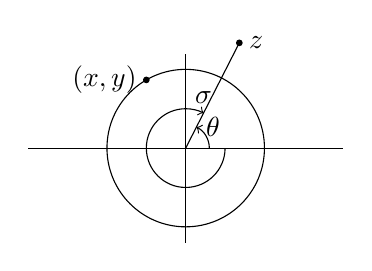
\begin{tikzpicture}
            \path (63: 1.5) coordinate (P);
            \path (120:1) coordinate (Q);
            \path (0: 0.3) coordinate (R);
            \path (0: 0.5) coordinate (R1);
            \draw (0, 0) ellipse (1cm and 1cm);
            \draw (-2, 0) -- (2, 0);
            \draw (0, -1.2) -- (0, 1.2);
            \filldraw[black] (P) circle (1pt) node[anchor=west] {$z$};
            \filldraw[black] (Q) circle (1pt) node[anchor=east] {$(x, y)$};
            \draw (0, 0) -- (P);
            \draw[->] (R) arc (0:63:0.3) node[anchor=west] {$\theta$};
            \draw[->] (R1) arc (360:63:0.5) node [anchor=south] {$\sigma$};
        \end{tikzpicture}
    \end{center}

    De esta forma, cualquier número complejo $z$ podrá expresarse como $z = \vabs{z}(\cos \theta, \sin \theta)$. Usualmente denominaremos a $\theta$ como el argumento de $z$, es decir, $\theta=\arg(z)$. Además, es común encontrar el módulo expresado con la letra $\rho$. Con esto podremos expresar $z$ como:\\
    $$
        z = \rho(\cos \theta, \sin \theta) = \rho(\cos \theta + i \sin \theta)
    $$

    Cuando definamos la exponencial compleja veremos que podemos expresar $z$ de la forma $z = \rho e^{i\theta}$.

    \begin{obs} %%TODO: Referenciar la imagen
        Como se aprecia en la figura superior, el argumento de $z$ no es único, tanto $\sigma$ como $\theta$ son el argumento de z (debido a que $\sigma = \theta - 2\pi$).\\

        Debido a que $\arg(z)$ es una función multievaluada (si $\arg(z) = \theta \implies \arg(z) = \sdf{\theta + 2n \pi \mid n \in \Z}$), en ocasiones querremos usar una función que escoja un solo argumento de ellos. La denominamos \textbf{argumento principal} ($\Arg{z}$), y la definimos restringiendo la imagen de $\arg{z}$ al intervalo $\left[0, 2\pi\right)$ o $\left[-\pi, pi\right)$.\\

        Sin embargo, aun habiendo determinado un argumento principal, en ninguno de los dos casos la función $\Arg()$ es continua en todo punto. Se puede ver que no existe una determinación continua del argumento.
    \end{obs}

    Esta forma de representar los números complejos nos simplificará varias tareas, como multiplicarlos o hallar raíces.
%%%%%%%%%%%%%%%%%%%%%%%%%%%%%%%%%%%%%%%%%%%%%%%%%%%%%%%%%%%%%%%%%%%%%%%%%% 30/01

    \begin{obs}
        Sea $\rho(\cos \theta, \sin \theta) = z = a + bi \implies \frac{b}{a} = \tan{\theta}$. Esto no significa que $\theta = \tan^{-1}\left(\frac{b}{a}\right)$ ya que la imagen de $\tan^{-1} \subseteq \left(-\frac{\pi}{2}, \frac{\pi}{2}\right)$.
    \end{obs}

    En general, encontrar el argumento de un número complejo no es tarea fácil, sin embargo en ciertos casos puede comprobarse a mano.

    \begin{eg}[Hallar la expresión polar de un número complejo. Hallar su inverso]
        Sea $z = 1-i \in \C$, vamos a hallar su expresión polar.
        $$
            \vabs{z} = \sqrt{1^2 + (-1)^2} = \sqrt 2
        $$
        Por tanto, $z = \sqrt{2} \cdot \left( \frac{1}{\sqrt 2} - \frac{i}{\sqrt 2} \right) = \sqrt 2 (\cos \theta + i \sin \theta)$. Resolviendo el sistema:
        \begin{align*}
            \cos \theta &= \frac{1}{\sqrt 2}\\
            \sin \theta &= - \frac{1}{\sqrt 2}
        \end{align*}
        Y al resolverlo hallamos $\theta = -\frac{\pi}{4}$ y entonces:
        $$
            z = \sqrt{2} (\cos \left(-\frac{\pi}{4}\right) + i \sin \left(-\frac{\pi}{4}\right))
        $$

        Si ahora queremos hallar su inverso, vamos a usar la identidad $z^{-1} = \frac{\cnj z}{\vabs{z}^2}$. Por tanto:
        $$
            z^{-1} = \frac{1}{2} (1 + i)
        $$
    \end{eg}

\subsection{Ra\'ices y potencias}

    Ya vimos al comienzo del capítulo que la forma de hallar la raíz cuadrada de un número complejo en la primera expresión que dimos del mismo era poco agradable. Podemos ver que la forma polar nos simplifica el cálculo.\\
    Para ello vamos a comenzar observando como se comporta la expresión polar frente a la multiplicación de complejos.\\

    Consideremos $z = \rho(\cos \theta, \sin \theta)$ y $w = \rho'(\cos \theta', \sin \theta')$. Entonces:
    $$
        z \cdot w = \rho \cdot \rho' (\cos \theta \cos \theta' - \sin \theta \sin \theta', \cos\theta \sin \theta' + \sin \theta \cos \theta') = \rho \cdot \rho' (\cos (\theta + \theta') + i\sin(\theta+\theta'))
    $$
    Es decir, cuando multiplicamos dos complejos en forma polar, el resultado es otro número complejo cuyo módulo es el producto de los módulos y el argumento es la suma de los argumentos. Esta propiedad simplifica el cálculo de raíces y potencias.

    \begin{eg}[Cálculo de una potencia de un número complejo]
        Sea $z = (\cos \theta, \sin \theta)$, entonces, usando lo que acabamos de ver:
        $$
            z^n = (\cos \theta, \sin \theta)^n = \cos(n\theta) + i \sin(n\theta)
        $$
    \end{eg}

    \begin{eg}[Cálculo de las raíces de un número complejo]
        Sean $z, w \neq 0 \in \C$, queremos resolver la ecuación $z^n = w$, es decir, encontrar las raíces n-ésimas de $w$.\\
        Podemos suponer que $w = \rho(\cos \theta + i \sin \theta)$ y $z = r (\cos t + i \sin t)$. Entonces queremos que:
        $$
            z^n = w \implies r^n (\cos(nt) + i \sin(nt)) =  \rho(\cos \theta + i \sin \theta)
        $$
        y entonces:
        \begin{align*}
            r &= \sqrt[n]{\rho}\\
            \theta + 2\pi k &= nt
        \end{align*}
        Simplificando la última identidad, obtenemos:
        $$
            t = \frac{\theta}{n} + 2\pi \frac{k}{n},\ k=0, \ldots, n-1
        $$
        y por tanto resultan $n$ raíces. (Para $k=n$ el complejo es el mismo que para $k = 0$).
    \end{eg}
% \section{Topolg\'ia del plano complejo}
% \section{Esfera de Riemann}
% \section{Funciones complejas}
% \section{L\'imites y continuidad}
